\documentclass{llncs}
\usepackage[latin1]{inputenc}
\usepackage{amsmath}
\usepackage{xspace}
\usepackage{amsfonts}
\usepackage{amssymb}
\usepackage{latexsym}
\usepackage{graphicx}
\usepackage[latin1]{inputenc}
\usepackage[noend]{algpseudocode}
\usepackage{url}
\usepackage{color}
\usepackage{fancyvrb}
\usepackage{mathpartir}
\usepackage{wrapfig}
\usepackage{caption}
\usepackage{subfigure}
\usepackage{tikz}
\usetikzlibrary{arrows,automata}
\usetikzlibrary{shapes.symbols}
\usetikzlibrary{shapes}

\newcommand{\calvin}{{\sc calvin}\xspace}
\newcommand{\QED}{{\sc qed}\xspace}
\newcommand{\civl}{{\sc civl}\xspace}
\newcommand{\boogie}{{\sc boogie}\xspace}
\newcommand{\zthree}{{\sc Z3}\xspace}
\newcommand{\casm}{{\sc casm}\xspace}
\newcommand{\why}{{\sc why}\xspace}

\renewcommand{\floatpagefraction}{0.75}

\makeatletter
\let\@copyrightspace\relax
\makeatother

\begin{document}

\title{Automated and modular refinement reasoning for concurrent programs}
\author{Chris Hawblitzel\inst{1} \and Erez Petrank\inst{2} \and Shaz Qadeer\inst{1} \and Serdar Tasiran\inst{3}}
\institute{Microsoft \and Technion \and Ko\c{c} University}

\maketitle


\newcommand{\Type}{\mathit{Type}}
\newcommand{\VarName}{\mathit{AllVar}}
\newcommand{\Var}{\mathit{Var}}
\newcommand{\Value}{\mathit{Value}}
\newcommand{\Expr}{\mathit{Expr}}
\newcommand{\StateExpr}{\mathit{Expr}}
\newcommand{\TransExpr}{\mathit{TransExpr}}
\newcommand{\LocalStateExpr}{\mathit{LocalExpr}}
\newcommand{\Spec}{\mathit{Spec}}
\newcommand{\Program}{\mathit{Program}}
\newcommand{\Prog}{\mathit{Prog}}
\newcommand{\ProcName}{\mathit{Proc}}
\newcommand{\ActionName}{\mathit{Action}}
\newcommand{\Proc}{\mathit{Proc}}
\newcommand{\proc}{\mathit{Pr}}
\newcommand{\Thread}{\mathit{Thread}}
\newcommand{\Body}{\mathit{Body}}
\newcommand{\Stmt}{\mathit{Stmt}}
\newcommand{\stmt}{\mathit{s}}
\newcommand{\locExpr}{\mathit{le}}
\newcommand{\exC}[1]{{\tt {#1}}}
\newcommand{\Frame}{F}
\newcommand{\Frames}{\overrightarrow{\Frame}}
\newcommand{\FrameCtxt}{\mathit{FC}}
\newcommand{\MakeFrames}[1]{\overrightarrow{#1}}

\newcommand{\ite}[3]{\mathit{if}\hspace{0.5mm}{#1}\hspace{0.5mm}\mathit{then}\hspace{0.5mm}{#2}\hspace{0.5mm}\mathit{else}\hspace{0.5mm}{#3}}
\newcommand{\while}[3]{\mathit{while}\hspace{0.5mm}\{#1\}\hspace{0.5mm}{#2}\hspace{0.5mm}\mathit{do}\hspace{0.5mm}{#3}}
\newcommand{\yield}[1]{\mathit{yield}\ #1}
\newcommand{\join}[1]{\mathit{join}\ #1}
\newcommand{\async}[1]{\mathit{async}\ #1}
\newcommand{\call}[1]{\mathit{call}\ #1}
\newcommand{\ablock}[2]{\mathit{ablock}\ {\{#1\}}\ {#2}\ }
\newcommand{\parcall}[2]{\mathit{call}\ {#1} || {#2}\ }
\newcommand{\assert}[1]{\mathit{assert}\ #1}
\newcommand{\assume}[1]{\mathit{assume}\ #1}
\newcommand{\havoc}[1]{\mathit{havoc}\ #1}
\newcommand{\goto}[1]{\mathit{goto}\ #1}
\newcommand{\fork}[1]{\mathit{par}\ #1}
\newcommand{\impl}[3]{ \{ {#1} \}  {#2} \preceq {#3} }
\newcommand{\skipstmt}{\mathit{skip}}
\newcommand{\hiddenVars}{\vec{h}}
\newcommand{\cf}{\mathit{cf}}
\newcommand{\state}{\sigma}
\newcommand{\unchangedExcept}[1]{\mathit{UnchangedExcept}_{ {#1} }}
\newcommand{\procs}{\mathit{ps}}

\newcommand{\Store}{\mathit{Store}}
\newcommand{\StoreGlobal}{\mathit{StoreGlobal}}
\newcommand{\StoreThreadLocal}{\mathit{StoreThreadLocal}}
\newcommand{\StoreLocal}{\mathit{StoreLocal}}
\newcommand{\varsG}{G}
\newcommand{\varsTL}{\mathit{TL}}
\newcommand{\varsL}{L}
\newcommand{\true}{\mathit{true}}
\newcommand{\false}{\mathit{false}}
\newcommand{\varsGTLL}{\varsG\cup\varsTL\cup\varsL}
\newcommand{\vars}{\sigma}
\newcommand{\PS}{\vec{\mathit{P}}}
\newcommand{\TS}{\overrightarrow{T}}
\newcommand{\LS}{\vec{\mathit{L}}}
\newcommand{\yielding}[1]{\mathit{yielding}(#1)}
\newcommand{\trans}{\longrightarrow}
\newcommand{\ytrans}{\hookrightarrow}
\newcommand{\ctrans}{\longmapsto}
\newcommand{\transmany}{\trans^{*}}
\newcommand{\xs}{\vec{\mathit{x}}}
\newcommand{\ws}{\vec{\mathit{w}}}
\newcommand{\ys}{\vec{\mathit{y}}}
\newcommand{\vs}{\vec{\mathit{v}}}
\newcommand{\ts}{\vec{\mathit{t}}}
\newcommand{\stmts}{\vec{\mathit{s}}}
\newcommand{\Collect}{\mathit{Collect}}
\newcommand{\Inv}{\mathit{Inv}}

\newcommand{\LinearVar}{\mathit{LinearVar}}
\newcommand{\lins}{\lambda}
\newcommand{\linss}{\vec{\lambda}}
\newcommand{\dom}{\mathit{dom}}
\newcommand{\cod}{\mathit{cod}}
\newcommand{\Global}{\mathit{Global}}
\newcommand{\Local}{\mathit{Local}}
\newcommand{\ThreadLocal}{\mathit{ThreadLocal}}

\newcommand{\Yields}{\mathit{Yields}}
\newcommand{\Ablocks}{\mathit{Ablocks}}
\newcommand{\requires}{\mathit{requires}}

\newcommand{\YieldingThread}{\mathit{YT}}
\newcommand{\YieldingThreads}{\overrightarrow{\YieldingThread}}
\newcommand{\bs}[1]{\overrightarrow{#1}}

\newcommand{\Vector}[1]{\overrightarrow{#1}}

\newcommand{\StmtCtxt}{\mathit{SC}}
\newcommand{\ThreadCtxt}{\mathit{TC}}
\newcommand{\ProgCtxt}{\mathit{PC}}
\newcommand{\CProgram}{\mathit{CProgram}}
\newcommand{\YProgram}{\mathit{YProgram}}

\newcommand{\error}{\mathit{error}}

\newcommand{\tl}{\mathit{tl}}
\newcommand{\tls}{\mathit{tls}}

\newcommand{\pre}{\mathit{pre}}
\newcommand{\post}{\mathit{post}}
\newcommand{\modvars}{\mathit{mod}}
\newcommand{\Continuation}{C}
\newcommand{\YieldingContinuation}{\mathit{YC}}

\newcommand{\jr}{\vdash_r}
\newcommand{\jy}{\vdash_y}
\newcommand{\jl}{\vdash_l}

\newcommand{\FH}[3]{\{#1\} #2 \{#3\}}
\newcommand{\RM}{\mathit{RM}}
\newcommand{\LM}{\mathit{LM}}

\newcommand{\pf}{\rightharpoonup}

\newcommand{\actions}{\mathit{as}}
\newcommand{\Refines}{\mathit{RS}}

\newcommand{\Mover}{\mathit{Mover}}

\newcommand{\accessVars}{\mathit{Acc}}

\newcommand{\FV}{\mathit{FV}}
\newcommand{\Same}{\mathit{Same}}
\newcommand{\Havoc}{\mathit{Havoc}}

\newcommand{\ABlockAny}{a}
\newcommand{\ABlockInside}{\mathrm{a^+}}
\newcommand{\ABlockOutside}{\mathrm{a^-}}

\newcommand{\ProcLins}{\mathit{ls}}
\newcommand{\linsmax}{\mathrm {MaxLinear}}

\newcommand{\mods}{M}
\newcommand{\AvailableActions}{\mathit{AS}}
\newcommand{\SkipProcs}{\mathit{SP}}

\newcommand{\MakeStore}[3]{{#1}\!\cdot\!{#2}\!\cdot\!{#3}}
\newcommand{\CommutativitySafe}{\mathit{CommutativitySafe}}
\newcommand{\InterferenceSafe}{\mathit{InterferenceSafe}}
\newcommand{\Yielding}{\mathit{Yielding}}
\newcommand{\Safe}{\mathit{Safe}}
\newcommand{\CSafe}{\mathit{CSafe}}
\newcommand{\Cooperative}{\mathit{Cooperative}}
\newcommand{\Injective}{\mathit{Injective}}

\newcommand{\Subst}{\Delta}
\newcommand{\Perm}{\mathit{Perm}}
\newcommand{\IsSet}{\mathit{IsSet}}
\newcommand{\old}{\mathit{old}}
\newcommand{\ga}[2]{{#1}\!\rightarrow\!{#2}}
\newcommand{\elim}[1]{\exists\exists {#1}}

\newcommand{\YSA}{\mathit{YSA}}


\begin{abstract}
We present \civl, a language and verifier for concurrent programs based on automated and modular refinement reasoning.  
\civl supports reasoning about a concurrent program at many levels of abstraction. 
Atomic actions in a high-level description are refined to fine-grain and optimized lower-level implementations. 
Modular specifications and proof annotations, such as location invariants and procedure pre- and post-conditions, 
are specified separately, independently at each level in terms of the variables visible at that level. 
We have implemented \civl as an extension to the \boogie language and verifier.
We have used \civl to refine a realistic concurrent garbage collection algorithm
from a simple high-level specification down to a highly-concurrent implementation described in terms of individual memory accesses.
\end{abstract}

\section{Introduction}
\label{sec:introduction}

We present a technique for verifying a refinement relation between two concurrent, shared-memory multithreaded programs. 
Our work is inspired by stepwise refinement~\cite{Wirth1971}, an approach in which a high-level description is systematically refined, 
potentially via several intermediate descriptions, down to a detailed implementation. 
This gives rise to the refinement verification problem of checking that a lower-level description correctly implements the abstract one -- a classical problem in verification.
For many systems, a natural way to write a full functional specification is to provide a description of the entire system at an abstract level. 
Checking refinement in this context is a means for full functional verification. 
Alternatively, a series of increasingly more abstract models of a system can be used to reduce the computational cost of verifying safety properties, since safety properties of higher-level models are preserved by lower-level models. 
This use of refinement is complementary to other techniques that combat the difficulty of verification, such as Floyd-Hoare, rely-guarantee, separation logic for modularity. 
The refinement problem has been investigated in many contexts ranging from checking correctness of implementations of cache-coherence protocols to verifying implementations of distributed algorithms. 
In the realm of sequential software, notable successes using the refinement approach include the work of Abrial et al.~\cite{AbrialBHHMV10} and the proof of full functional correctness of the seL4 microkernel~\cite{KleinAEMSKH14}. 
For shared-memory multithreaded software, there has only been limited, application-specific study of refinement. 
Examples are approaches to checking linearizability of concurrent data structures and some manual proofs of garbage collectors. 
A generic, widely-applicable approach to specifying and verifying refinement for shared-memory concurrent software is lacking. 


A key challenge in specifying and verifying multi-threaded software, differently from sequential software, is that procedures are not a clean factoring of a program into modules. 
For sequential software, in the popular software verification approach based on the method of Floyd~\cite{Floyd67} and Hoare~\cite{Hoare69}, the verification of a large software component is performed modularly by verifying each procedure in it separately.
This modularity is enabled by the use of interface specifications (preconditions and postconditions) constraining the behavior of each procedure.
It is well-known that the Floyd-Hoare method is difficult to generalize to reasoning about concurrent shared-memory programs,
primarily because the execution of a procedure may be interfered with by concurrently executing threads.
Several attempts have been made to extend Floyd-Hoare reasoning to deal with concurrent interference, 
including classical approaches such as location invariants~\cite{Ashcroft75,OwickiG76} and rely-guarantee~\cite{Jones83},
and other more recent approaches~\cite{OHearn07,RGSep}. 
In this paper, our goal is orthogonal and complementary to these approaches; We provide a methodology in which the {\em refinement} problem can be stated in a modular way guided by the syntactic structure of the program as in the Floyd-Hoare method. 
We further strive to make the verification of refinement as similar in spirit to the Floyd-Hoare approach as possible. 
We check refinement by reasoning about the code of a single procedure at a time, in fact, one interference-free step of the implementation at a time. 

In this paper, we introduce the \civl approach to reasoning about concurrent shared-memory software.
In the \civl approach, a program is described as a collection of procedures whose implementation 
can use the standard features such as assignment, conditionals, loops, procedure calls, and thread creation. 
Each procedure accesses shared global variables only through invocations of atomic actions.
During a refinement step, a subset of the atomic actions may be refined by new procedures and a new program is 
obtained by replacing the invocation of an atomic action by a call to the corresponding procedure refining the action.
Several such steps may be performed one after another until all atomic actions in the final program are directly implementable primitives.
This process may be carried out in a bottom-up rather than top-down fashion, in which case an atomic action 
can be thought of as the specification of the procedure that implements it.
Unlike classical program verifiers based on Floyd-Hoare reasoning that manipulate a program and annotations, 
the \civl verifier manipulates multiple operational descriptions of a program, i.e., several levels of refinement are specified and verified at once. 

In \civl, approximately speaking, a program refines another when there is a simulation relation connecting the two programs. 
The existence of such a simulation relation is inferred from per-procedure checks that relate the atomic specification and the code implementing a procedure. 
In this check, the abstract system (a two-state automaton) takes some stuttering steps, followed by the atomic action, followed by some more stuttering steps. 
Interference on shared state is modeled by the procedure pre- and post-condition predicates during stuttering steps before and after the atomic action, respectively. 
The verifier checks that, for each control path through the body of the implementation code, the program state sequences that this control path gives rise to are simulated by the specification automaton. 
More specifically, the control path is divided into ``steps'' (possibly consisting of more than one atomic action, explained below) where each step must map to a stuttering transition in the specification, except one, which maps to the atomic action specification.
To be able to carry out syntactically-decomposed reasoning on the implementation code in this manner, formulating per path and per step checks guided by the syntactic structure, we needed to address the following issues. 
\begin{itemize}
\item We need to define ``steps''. This has consequences in terms of the number of checks that need to be performed, and the number of user annotations in the procedure body.
\item The code for a ``step'' typically does not refine a stuttering action or the atomic action specification in a vacuum. A pre-condition for the step in terms of shared variables is needed. The per-step pre-conditions need to be correct, satisfied by the larger program.
\end{itemize}
We now discuss these issues. 

An important innovation in \civl addresses the first issue of defining the ``steps''. While proving refinement,
reasoning is done on an operational semantics that is {\em cooperative\/} rather than {\em preemptive\/}.
The preemptive semantics is the usual sequentially consistent semantics of shared-memory concurrency in which all threads are imagined
to execute on a single processor and preemption, which causes a thread to be scheduled out and a nondeterministically chosen thread to 
be scheduled in, may occur before any instruction.\footnote{In this paper, 
we focus our attention on sequential consistency and leave consideration of weak memory models to future work.}
The cooperative semantics is explicitly introduced by the programmer through the use of a new primitive {\em yield\/} statement;
in this semantics a thread can be scheduled out only when it is about to execute a yield statement.

Given a program $Q$ and the program $P$ obtained by replacing each invocation of an atomic action in $P$ 
with the procedure that refines it, the \civl verifier provides two guarantees.
First, it guarantees that the safety of the cooperative semantics of $P$ implies the safety of the preemptive semantics of $P$.
This verification is done by computing a automata-theoretic simulation check~\cite{HenzingerHK95} 
on an abstraction of $P$ that interprets each atomic action invoked by $P$ 
as a member of a finite set of mover types~\cite{Lipton75,FlanaganFLQ08}.
Second, it guarantees that every cooperative execution of $P$ is simulated by a preemptive execution of $Q$.
This check is performed in a syntactically-decomposed manner as referred to above, by calculating logical verification conditions from the bodies of procedures in $P$ and 
verifying them with an automated theorem prover~\cite{MouraB08}.
These two checks together guarantee that the 
safety of the preemptive semantics of $Q$ implies the safety of the preemptive semantics of $P$.

\civl's solution to the second issue, the fact that per ``step'' refinement verification typically requires invariants about the program execution, is to allow the programmer to specify location-specific invariants, attached either to a yield statement
or as a precondition or a postcondition of a procedure. 
The collection of such location invariants, placed as annotations in all refined procedures, must be correct as a whole and each  annotation must continue to hold in spite of potential interference from concurrently executing threads.
The problem of formulating the correctness of such a collection of annotations happens to be dealt in the work of Owicki and Gries~\cite{OwickiG76}. Differently, here we do not need the annotations to be strong enough to prove program correctness, but only strong enough to provide the context for per-procedure refinement checking. 
To reduce the annotations required for logical non-interference checking, 
the \civl verifier also provides a linear type system~\cite{Wadler90lineartypes} 
that allows logical encoding of thread identifiers, permissions~\cite{boyland:03fractions}, 
and disjoint memory~\cite{LahiriQW11}.

We have implemented \civl as a conservative extension of the \boogie verifier.  
We have used it to verify a collection of microbenchmarks and benchmarks from the literature such as
the ticket algorithm~\cite{ticket}, Treiber stack~\cite{treiber}, work-stealing queue~\cite{wsq},
device cache~\cite{device-cache}, and lock-protected increment~\cite{incr}.
We have also verified a concurrent garbage collector algorithm (say something more here).

We conclude this section by summarizing the novel features of the \civl verifier:
\begin{itemize}
\item Automated refinement checking of atomic action specifications against imperative code.
\item A combination of automata-theoretic checking based on simulation relations and logical checking based on verification conditions.
\item Powerful and flexible invariant reasoning based on location-specific invariants and linear variables.
\end{itemize}
The \civl verifier is the first to put these features together and use them to verify a collection of realistic and challenging shared-memory
concurrent programs.

\section{Overview}
\label{sec:overview}

We present an overview of our approach to refinement on the program in Figure~\ref{fig:reft},
a simplified version of the write barrier in a concurrent garbage collector (GC).
In a concurrent GC, a color (either \exC{WHITE}, \exC{GRAY}, or \exC{BLACK})
is associated with each object on the heap.  
Before writing to an address \exC{addr}, a mutator executes a write
barrier. It checks 
\exC{addr} has color \exC{WHITE}
and sets it to \exC{GRAY}, indicating that the object at \exC{addr}
and objects reachable from it should not be garbage collected. 

\begin{wrapfigure}[25]{l}{0.5\textwidth}
\vspace*{-1cm}
{\scriptsize
\begin{verbatim}
var Color: int; // WHITE=1, GRAY=2, BLACK=3

procedure WB(linear tid:Tid)
atomic [if (Color == WHITE) Color := GRAY];
ensures Color >= GRAY;
{
  var cNoLock:int;
  cNoLock := GetColorNoLock(tid);
  yield Color >= cNoLock;
  if (cNoLock == WHITE) 
    call WBSlow(tid);
}

procedure WBSlow(linear tid:Tid)
atomic [if (Color == WHITE) Color := GRAY];
{
  var cLock:int;
  call AcquireLock(tid);
  cLock := GetColorLocked(tid);
  if (cLock == WHITE) 
    call SetColorLocked(tid, GRAY);
  call ReleaseLock(tid);
}

procedure GetColorNoLock(linear tid:Tid) 
  returns (cl:int) atomic [...];
procedure AcquireLock(linear tid:Tid) 
  right [...];
procedure ReleaseLock(linear tid:Tid) 
  left [...];
procedure GetColorLocked(linear tid:Tid) 
  returns (cl:int) both [...];
procedure SetColorLocked(linear tid:Tid, 
  cl: int) atomic [...];
\end{verbatim}
}
\vspace*{-0.3cm}
\caption{Write barrier}
\label{fig:reft}
\end{wrapfigure}

Procedure \exC{WB} implements the write barrier.
To simplify exposition, 
we consider a single object whose color is stored in the shared variable \exC{Color}.
\exC{WB} first reads \exC{Color} without holding a lock, to avoid,
when possible, the
cost of acquiring and releasing a lock for each address encountered by
a mutator. 
If \exC{Color} is {\tt WHITE}, it calls the more expensive procedure \exC{WBSlow} 
to re-examines and possibly update \exC{Color} while holding the
lock. The annotation \exC{yield} \exC{Color >= cNoLock} is a local invariant
expected to be preserved by the environment of the \exC{WB} procedure. 
\civl simplifies reasoning about \exC{WB} and \exC{WBSlow} by allowing us to 
compactly express their specification as the following atomic action:\\
\begin{small}
\begin{tt}
[if (Color == WHITE)  Color := GRAY]
\end{tt}
\end{small}\\
This specification indicates that regardless of the different implementations of 
\exC{WB} and \exC{WBSlow} and regardless of how the environment interferes
with their execution, to their respective callers it appears as if they atomically execute the above code.

{\bf Per-procedure simulation, non-interference via invariants.}
The correctness of \exC{WB} is not obvious, and its verification
requires a combination of techniques as discussed next. 
Consider the following potential scenario. 
\exC{WB}, not holding a lock, reads {\tt Color} and
sets \exC{cNoLock} to \exC{GRAY} and then yields. Another thread sets {\tt Color} to
{\tt WHITE}. \exC{WB} resumes, but does nothing and exits,
because the procedure-local variable \exC{cNoLock} is \exC{GRAY}. In this scenario, the atomic action
specification of \exC{WB} would not be satisfied. However, in the GC this
scenario is not possible. 
The yield predicate (location invariant) expresses the fact that
other threads in the environment of the thread running \exC{WB} can
only modify {\tt Color} to a higher (darker) value -- \civl verifies the correctness
of this location invariant.
Using this location invariant, \civl then verifies atomicity
refinement for {\tt WB} by verifying the existence of a particular
simulation-relation. Each control path through \exC{WB} is analyzed as
a sequence of code fragments, from one {\tt yield} statement to the
next. For each control path, exactly one of these fragments is simulated by the atomic action specification and other fragments do not modify
global state. 
This proof requires both correct modeling of environment interference in the yield predicate
and the atomic action specification for the called procedure \exC{WBSlow}.
The \civl verifier automatically computes a logical verification condition capturing
these proof obligations from the body and specification of \exC{WB}.

Just as the verification of \exC{WB} builds on the specification of \exC{WBSlow},
the verification of \exC{WBSlow} builds on other refinement proofs (not shown) 
of the procedures called in \exC{WBSlow};
these procedures are shown at the bottom of the figure. 
This example shows only one procedure at this layer. In programs
with many procedures with atomic specifications at each layer,
\civl combines the per-procedure refinement proofs soundly into a
whole-program refinement proof. 

{\bf Reduction, preemptive vs cooperative semantics.}
The verification of \exC{WBSlow} highlights reduction-related features
in \civl. 
Refinement checking is performed on cooperative semantics in which a 
{\tt yield}-to-{\tt yield} execution fragment of code is executed atomically.
However, in a real execution, control can switch between threads at any point in the code. 
A naive modeling of a real execution would put a yield statement before every instruction in the code.
The absence of a yield statement before every instruction is justified by reasoning about mover types~\cite{FlanaganFLQ08}. 
The procedures called in \exC{WBSlow} have the mover types claimed in their
declarations and verified by \civl. 
For example, the mover type of \exC{Acquirelock} is {\tt right} which indicates 
that it commutes later in time against concurrently executing
environment actions. 
% \exC{ReleaseLock} has mover type {\tt left} and it commutes earlier in time;
% \exC{SetColorLocked} has mover type {\tt atomic} and it does not commute;
% \exC{GetColorLocked} has mover type {\tt both} and it commutes both earlier and later in time.
These mover types are checked by constructing verification conditions from each pair of atomic actions.

The use of movers is entirely optional in \civl, but very beneficial
in our experience. One can avoid 
mover and commutativity reasoning, simply
annotating atomic action specifications with the mover type {\tt atomic}.
However, without mover reasoning,  a yield statement and an
accompanying predicate
must be inserted before every invocation of an atomic action.
It has been demonstrated in work in the literature that mover
reasoning simplifies many proofs~\cite{ElmasQT09}. 
In our experience with \civl, we have observed that using more yield
predicates rather than mover reasoning can make proofs difficult in two ways.
\begin{wrapfigure}[8]{l}{0.5\textwidth}
\vspace*{-1cm}
\begin{center}
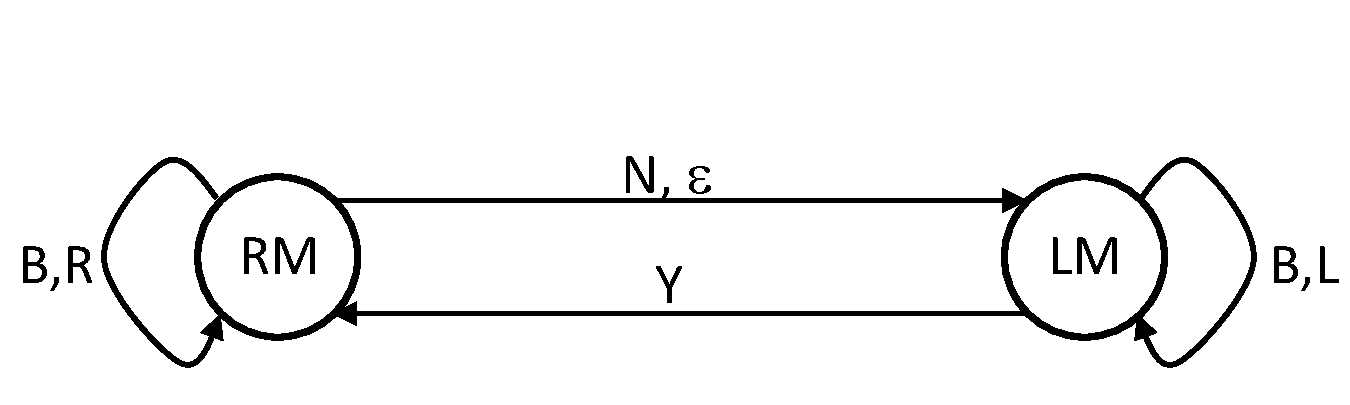
\includegraphics[scale=0.25]{YieldTypeCheckingAutomaton.pdf}
\end{center} 
\vspace*{-0.3cm}
\caption{Yield sufficiency automaton ($YSA$)}
\label{fig:ysa}
\end{wrapfigure}
First, the annotation burden goes up because sophisticated ghost variables may need to be introduced in the 
program semantics.\footnote{Location invariants that cannot refer to the state of other threads are known to be incomplete, 
both in theory and in practice.}
Second, the computational cost of the pairwise mover reasoning is replaced by the cost of pairwise non-interference checks between yield predicates 
and concurrently executing atomic actions. 
\civl does not force the use of mover
reasoning but provides automation for this important verification
feature and its use in conjunction with other techniques illustrated in
this section. 

Given verified mover types for actions, \civl verifies reduction, i.e., the correctness of the placement of {\tt yield}s using a novel  approach.
A {\em yield sufficiency automaton\/} ($\YSA$ in Figure~\ref{fig:ysa})
encodes all sequences of atomic actions (of {\bf R}ight, {\bf L}eft,
{\bf B}oth and
{\bf N}on-mover types)  and yields for which safety of cooperative semantics is sufficient 
for safety of preemptive semantics. 
\begin{wrapfigure}[8]{l}{0.5\textwidth}
\vspace*{-1cm}
\begin{center}
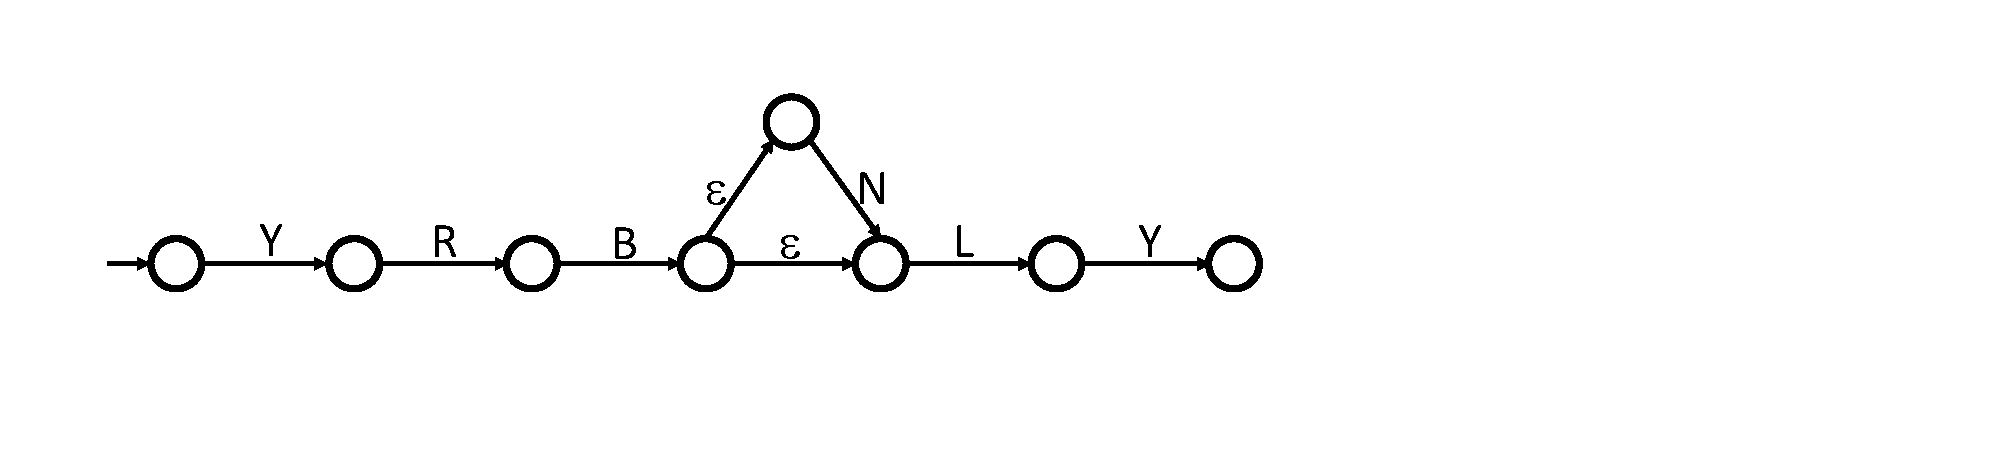
\includegraphics[scale=0.25]{WBSlow.pdf}
\end{center}
\vspace*{-0.5cm}
\caption{Abstraction of \exC{WBSlow}}
\label{fig:midwb}
\end{wrapfigure}
Each ``transaction'' starts with a sequence of right movers (or both movers) and ends with a sequence of left movers (or both movers).
In the middle, it can have at most one non mover. Transactions must be
separated by {\tt yield}s.
\civl then interprets the control-flow graph of each procedure as an automaton with mover types as edge labels. 
This abstraction for \exC{WBSlow} is shown in Figure~\ref{fig:midwb}.
\civl verifies that this automaton is simulated by the yield sufficiency automaton using an existing algorithm for computing simulation relations~\cite{HenzingerHK95}.

{\bf Linear variables.}
In Figure~\ref{fig:reft}, thread identifier (\exC{tid}) variables are declared \exC{linear} to indicate that two threads cannot possess the same thread identifier simultaneously.
To enforce unique ownership of linear resources, the \civl type checker prohibits duplication of linear resources~\cite{Wadler90lineartypes}.
Interference checking and commutativity checking leverage this linearity by automatically inserting assumptions about disjointness of linear resources into verification conditions,
making it easier to prove non-interference and commutativity.
Linearity is general enough to support much more than just fixed thread identifiers:
\civl also uses it to express separation of memory (as is done
commonly in separation logic proofs~\cite{Reynolds02}; see \cite{LahiriQW11})
and to express permissions~\cite{boyland:03fractions} that may be transferred but not duplicated between threads.
Our verified GC, for example, expresses mutual exclusion during initialization and root scanning by temporarily transferring permissions from mutator threads to the GC thread.

{\bf Variable hiding.}
The atomic action specification of \exC{WBSlow} makes no reference to the lock variable, although its implementation involves a lock. 
When verifying refinement for \exC{WBSlow}, the lock variable has been hidden. 
\civl allows the programmer to both introduce and hide variables in
each refinement step, thereby providing the capability to perform data refinement.
The ability to introduce and hide variables and write yield predicates specific to each refinement step 
facilitates proofs spanning a large range of abstraction.


\begin{figure}
\setlength{\tabcolsep}{3pt}
{\bf Program Syntax} \\
\begin{tabular}{rclcl}
$g$ & $\in$ & $\Globals \subseteq \VarName$ \\
$\tl$ & $\in$ & $\ThreadLocals \subseteq \VarName$ \\
$l$ & $\in$ & $\Locals \subseteq \VarName$ \\
$x,y$ & $\in$ & $\Var = \Globals \cup \ThreadLocals \cup \Locals$ \\
$t$ & $\in$ & $\Type$ \\
$v$ &  $\in$ & $\Value$ \\
$e, \phi, \psi, \rho$ & $\in$ & $\StateExpr$ \\
$\alpha, \beta$ & $\in$ & $\TransExpr$ \\
$\locExpr$ & $\in$ & $\LocalStateExpr$ \\
$P$ & $\in$ & $\ProcName$ \\
$A$ & $\in$ & $\ActionName$ \\
$\bodies$ & $\in$ & $\ProcName \rightarrow \Stmt$ \\
$m$ & $\in$ & $\Mover = \{B,R,L,N\}$\\
$\actions$ & $\in$ & $\ActionName \rightarrow (\StateExpr, \TransExpr, \Mover)$ \\
$\specs$ & $\in$ & $\ProcName \rightarrow (\StateExpr, \StateExpr)$ \\
$\refines$ & $\in$ & $\ProcName \pf \ActionName$ \\
$H$ & $\in$ & $2^{\ThreadLocals \cup \Globals}$ \\
$\varsG$ & $\in$ & $ \Globals \rightarrow \Value$ \\
$\varsTL$ & $\in$ & $ \ThreadLocals  \rightarrow \Value$ \\
$\varsL$ & $\in$ & $ \Locals \rightarrow \Value$ \\
$\sigma$ & $\in$ & $ \Var \rightarrow \Value$ \\
$\Gamma$ & $\in$ & $ \Var \rightarrow \Type$ \\
$\lins$ & $\in$ & $2^{\Var}$ \\
\end{tabular}
~\\
~\\
\begin{tabular}{rclcl}
$\stmt \in \Stmt$ &::= & $\skipstmt \mid \assert{\locExpr} \mid \yield{e} \mid$ \\
                  & & $\call{A} \mid \call{P} \mid \async{P} \mid $\\
                  & & $\ablock{e}{s} \mid s;\;s \mid$\\
                 & & $\ite{\locExpr}{s}{s} \mid$ \\
                  & & $\while{e}{\locExpr}{s}$ \\ 
$\StmtStack \in \mathit{StmtStack}$ &::= & $\stmt \mid (\varsL,\StmtStack) \mid \StmtStack;\stmt$ \\
$T \in \mathit{Thread}$ &::= &$(\varsTL, (\varsL, \StmtStack))$ \\
\\
$\StmtCtxt \in \mathit{StmtCtxt}$ &::= &$[]_{Stmt} \mid \StmtCtxt;\stmt$ \\
$\StmtStackCtxt \in \mathit{StmtStackCtxt}$ &::= & $([]_{\Locals}, \StmtCtxt) \mid (L,\StmtStackCtxt) \mid \StmtStackCtxt;\stmt$ \\
$\ThreadCtxt \in \mathit{ThreadCtxt}$ &::= &$([]_{\ThreadLocals}, ([]_{\Locals}, \StmtCtxt)) \mid$ \\
 & &$([]_{\ThreadLocals}, (\varsL, \StmtStackCtxt))$ \\
$\YieldingThread \in \mathit{YieldingThread}$ &::= &$\ThreadCtxt[\varsTL][\varsL][\yield{e}]$ \\
$\ProgCtxt \in \mathit{ProgCtxt}$ &::= &$\YieldingThreads \cdot \ThreadCtxt \cdot \YieldingThreads$ \\
\end{tabular}
~\\
~\\
\begin{tabular}{rcl}
$\Prog$ & $\in$ & $\Program = (\bodies, \actions, \specs, \refines, H, \varsG, \TS)$ \\
\end{tabular}
\setlength{\tabcolsep}{6pt}
\caption{Syntax}
\label{fig:syntax}
\end{figure}

\begin{figure}
\scriptsize{
\medskip
%%%%%%%%%%%%%%%%%%%%
$
\inferrule
{
\vdash (\varsG\cup\varsTL\cup\varsL, s) \trans (\varsG'\cup\varsTL'\cup\varsL', s')
}
{\vdash (\varsG, \ProgCtxt[\varsTL][\varsL][s]) \trans (\varsG', \ProgCtxt[\varsTL'][\varsL'][s'])}
\;(\textsc{Program-Step})
$
\medskip
%%%%%%%%%%%%%%%%%%%%
$
\inferrule
{
\vdash (\varsG\cup\varsTL\cup\varsL, s) \fails
}
{\vdash (\varsG, \ProgCtxt[\varsTL][\varsL][s]) \fails}
\;(\textsc{Program-Fail})
$
\medskip
%%%%%%%%%%%%%%%%%%%%
$
\inferrule
{
\specs(P) = (\phi, \psi) \\ T' = (\varsTL, (\varsL, \yield{\phi};\bodies(P)))
}
{\vdash (\varsG, \ProgCtxt[\varsTL][\varsL][\async{P}]) \trans (\varsG, \ProgCtxt[\varsL][\skipstmt] \cdot T')}
\;(\textsc{Async})
$
\medskip
%%%%%%%%%%%%%%%%%%%%
$
\inferrule
{
\\
}
{\vdash (\varsG, \YieldingThreads \cdot (\varsTL, (\varsL,\skipstmt)) \cdot \YieldingThreads') \trans (\varsG, \YieldingThreads \cdot \YieldingThreads')}
\;(\textsc{Thread-End})
$
\medskip
%%%%%%%%%%%%%%%%%%%%
$
\inferrule
{
\specs(P) = (\phi, \psi)
}
{\vdash (\varsG, \ProgCtxt[\varsTL][\varsL][\call{P}]) \trans (\varsG, \ProgCtxt[\varsTL][\varsL][\Frame{L}{\yield{\phi};\bodies(P);\yield{\psi}}])}
\;{(\textsc{Call})}
$
\medskip
%%%%%%%%%%%%%%%%%%%%
$
\inferrule
{
\\
}
{\vdash (\varsG, \ProgCtxt[\varsTL][\varsL][\Frame{\varsL'}{\skipstmt}]) \trans (\varsG, \ProgCtxt[\varsTL][\varsL][\skipstmt])}
\;{(\textsc{Return})}
$
%%%%%%%%%%%%%%%%%%%%
}
\caption{Operational semantics for program}
\label{fig:operational-semantics1}
\end{figure}


\begin{figure}
\scriptsize{
\medskip
\medskip
%%%%%%%%%%%%%%%%%%%%
$
\inferrule
{
\vars \vdash \locExpr \rightarrow \true
}
{\vdash (\vars, \assert{\locExpr}) \trans (\vars, \skipstmt)}
\;{(\textsc{Assert-True})}
$
\medskip
%%%%%%%%%%%%%%%%%%%%
$
\inferrule
{
\vars \vdash \locExpr \rightarrow \false
}
{\vdash (\vars, \assert{\locExpr}) \fails}
\;{(\textsc{Assert-False})}
$
\medskip
%%%%%%%%%%%%%%%%%%%%
$
\inferrule
{
\actions(A) = (\rho, \alpha, m) \\
(\vars, \vars') \vdash \alpha \\
}
{
\vdash (\vars, \call{A}) \trans (\vars',\skipstmt)
}
\;{(\textsc{Atomic})}
$
\medskip
%%%%%%%%%%%%%%%%%%%%
$
\inferrule
{
\\
}
{\vdash (\vars, \yield{e}) \trans (\vars, \skipstmt)}
\;{(\textsc{Yield})}
$
\medskip
%%%%%%%%%%%%%%%%%%%%
$
\inferrule
{
\vars \vdash e \rightarrow \true
}
{\vdash (\vars, \ablock{e}{\stmt}) \trans (\vars, \stmt)}
\;{(\textsc{AtomicBlock})}
$
\medskip
%%%%%%%%%%%%%%%%%%%%
$
\inferrule
{
\\
}
{\vdash (\vars, \skipstmt;\stmt) \trans (\vars, \stmt)}
\;{\;\;\;\;\;\;\;\;\;\;\;\;(\textsc{Seq})}
$
\medskip
%%%%%%%%%%%%%%%%%%%%
$
\inferrule
{
\vars \vdash \locExpr \rightarrow \mathit{true}
}
{\vdash (\vars, \ite{\locExpr}{s_1}{s_2}) \trans (\vars, s_1)}
\;{(\textsc{If-True})}
$
\medskip
%%%%%%%%%%%%%%%%%%%%
$
\inferrule
{
\vars \vdash \locExpr \rightarrow \mathit{false}
}
{\vdash (\vars, \ite{\locExpr}{s_1}{s_2}) \trans (\vars, s_2)}
\;{(\textsc{If-False})}
$
\medskip
%%%%%%%%%%%%%%%%%%%%
$
\inferrule
{
\vars \vdash \locExpr \rightarrow \mathit{false}
}
{\vdash (\vars, \while{e}{\locExpr}{s}) \trans (\vars, \skipstmt)}
\;{(\textsc{While-False})}
$
\medskip
%%%%%%%%%%%%%%%%%%%%
$
\inferrule
{
\vars \vdash \locExpr \rightarrow \mathit{true}
}
{\vdash (\vars, \while{e}{\locExpr}{s}) \trans (\vars, s;\while{e,m}{\locExpr}{s})}
\;{(\textsc{While-True})}
$
%%%%%%%%%%%%%%%%%%%%
}
\caption{Operational semantics for statement}
\label{fig:operational-semantics2}
\end{figure}

%%% Local Variables: 
%%% mode: latex
%%% TeX-master: "paper"
%%% End: 



\subsection{Type checking}
\begin{figure*}
\scriptsize{
\medskip
%%%%%%%%%%%%%%%%%%%%
$
\inferrule
{
}
{
\lins;\ABlockAny \vdash \skipstmt : \lins
}
\;(\textsc{Skip})
$
\medskip
%%%%%%%%%%%%%%%%%%%%
$
\inferrule
{
}
{
\lins;\ABlockOutside \vdash \assert{\locExpr} : \lins
}
\;(\textsc{Assert})
$
\medskip
%%%%%%%%%%%%%%%%%%%%
$
\inferrule
{
\lins_y \subseteq \lins
}
{
\lins;\ABlockOutside \vdash \yield{e,\lins_y} : \lins
}
\;(\textsc{Yield})
$
\medskip
%%%%%%%%%%%%%%%%%%%%
$
\inferrule
{
\ProcLins(A) = (\lins,\lins')
}
{
\lins;\ABlockInside \vdash \call{A} : \lins'
}
\;(\textsc{Atomic})
$
\medskip
%%%%%%%%%%%%%%%%%%%%
$
\inferrule
{
\ProcLins(P) = (\lins,\lins') \\
}
{
\lins;\ABlockOutside \vdash \call{P} : \lins'
}
\;(\textsc{Proc})
$
\medskip
%%%%%%%%%%%%%%%%%%%%
$
\inferrule
{
\lins_G \subseteq \Global \\
\lins \cup \lins_P \cup \lins_P' \subseteq \ThreadLocal \\
\ProcLins(P) = ((\lins_G,\lins_P),(\lins_G,\lins_P')) \\
}
{
\lins_G,\lins,\lins_P;\ABlockOutside \vdash \async{P} : \lins_G,\lins
}
\;(\textsc{Async})
$
\medskip
%%%%%%%%%%%%%%%%%%%%
$
\inferrule
{
\lins;\ABlockInside \vdash \stmt : \lins' \\
\lins_a \subseteq \lins
}
{
\lins;\ABlockOutside \vdash \ablock{e,\lins_a}{\stmt} : \lins'
}
\;(\textsc{Ablock})
$
\medskip
%%%%%%%%%%%%%%%%%%%%
$
\inferrule
{
\lins;\ABlockAny \vdash \StmtStack : \lins'
}
{
\lins;\ABlockAny \vdash (\varsL,\StmtStack) : \lins'
}
\;(\textsc{Stack})
$
\medskip
%%%%%%%%%%%%%%%%%%%%
$
\inferrule
{
\lins;\ABlockAny \vdash \StmtStack : \lins' \\
\lins';\ABlockAny \vdash \stmt : \lins''
}
{
\lins;\ABlockAny \vdash \StmtStack;\stmt : \lins''
}
\;(\textsc{Seq})
$
\medskip
%%%%%%%%%%%%%%%%%%%%
$
\inferrule
{
\lins;\ABlockAny \vdash s_1 : \lins' \\
\lins;\ABlockAny \vdash s_2 : \lins'
}
{
\lins;\ABlockAny \vdash \ite{\locExpr}{s_1}{s_2} : \lins'
}
\;(\textsc{Ite})
$
\medskip
%%%%%%%%%%%%%%%%%%%%
$
\inferrule
{
\lins;\ABlockAny \vdash s : \lins
}
{
\lins;\ABlockAny \vdash \while{e,\alpha}{\locExpr}{s} : \lins
}
\;(\textsc{While})
$
\medskip
%%%%%%%%%%%%%%%%%%%%
$
\inferrule
{
\ProcLins(P) = (\lins,\lins') \\
\procs(P) = (\phi, \mods, \psi, \stmt) \\
\lins;\ABlockOutside \vdash \stmt : \lins'
}
{
\vdash P
}
\;(\textsc{Procedure})
$
\medskip
%%%%%%%%%%%%%%%%%%%%
$
\inferrule
{
T = (\varsTL, (\varsL, \StmtStack)) \\
\lins;\ABlockOutside \vdash \StmtStack : \lins'
}
{
\lins \vdash T
}
\;(\textsc{Thread})
$
\medskip
%%%%%%%%%%%%%%%%%%%%
$
\inferrule
{
\ProcLins(A) = (\lins,\lins') \\
\lins \cap \Global = \lins' \cap \Global \\
\actions(A) = (\rho, \alpha, m) \\\\
\forall (\sigma,\sigma') \in \alpha.
  \disjoint(\{\sigma(x) \mid x \in \lins\}) \wedge
  \disjoint(\{\sigma'(x) \mid x \in \lins'\}) \\
\forall (\sigma,\sigma') \in \alpha.
  \bigcup\{\sigma'(x) \mid x \in \lins'\} \subseteq \bigcup\{\sigma(x) \mid x \in \lins\}
}
{
\vdash A
}
\;(\textsc{Action})
$
\medskip
%%%%%%%%%%%%%%%%%%%%
$
\inferrule
{
\forall P \in \ProcName. \vdash P \\
\forall A \in \ActionName. \vdash A \\
\lins_G \subseteq \Global \\
\forall 1 \le i \le n. (\lins_G,\lins_i \vdash T_i) \\
\forall 1 \le i \le n. (\lins_i \subseteq \ThreadLocal) \\
\forall 1 \le i \le n. (T_i = (\varsTL_i, \ldots)) \\
\disjoint(\{\varsG(x) \mid x \in \lins_G\} \cup
  \{\varsTL_i(x) \mid 1 \le i \le n, x \in \lins_i\})
}
{
\vdash (\procs, \actions, \ProcLins, \varsG, T_1 \ldots T_n)
}
\;(\textsc{Program})
$
\medskip
%%%%%%%%%%%%%%%%%%%%
}
\caption{Type checking rules}
\label{fig:type-checking}
\end{figure*}

\subsection{Safety}
\begin{figure}
\scriptsize{
\medskip
%%%%%%%%%%%%%%%%%%%%
$
\inferrule
{
}
{\procs;\actions;\RefinementAny;\{\} \jp \FH{\phi}{\skipstmt}{\phi}}
\;(\textsc{Skip})
$
\medskip\\
%%%%%%%%%%%%%%%%%%%%
$
\inferrule
{
}
{\procs;\actions;\RefinementOutside;\{\} \jp \FH{\phi}{\assert{\locExpr}}{\phi}}
\;(\textsc{Assert1})
$
\medskip
%%%%%%%%%%%%%%%%%%%%
$
\inferrule
{
}
{\procs;\actions;\RefinementInside;\{\} \jp \FH{\phi \wedge \locExpr}{\assert{\locExpr}}{\phi}}
\;(\textsc{Assert2})
$
\medskip
%%%%%%%%%%%%%%%%%%%%
$
\inferrule
{
}
{\procs;\actions;\RefinementAny;\{\} \jp \FH{e}{\yield{e,\lins}}{e}}
\;(\textsc{Yield})
$
\medskip
%%%%%%%%%%%%%%%%%%%%
$
\inferrule
{
\actions(A) = (\rho, \alpha, m) \\ 
\mods \subseteq \ThreadLocal \\
\alpha \Rightarrow \Havoc(\Global \cup \mods \cup \Local) \\
\phi \Rightarrow \rho \\ 
\Unsat{\phi \circ \alpha \circ \neg \psi} \\
}
{\procs;\actions;\RefinementAny;\mods \jp \FH{\phi}{\call{A}}{\psi}}
\;(\textsc{Atomic})
$
\medskip
%%%%%%%%%%%%%%%%%%%%
$
\inferrule
{
\procs(P) = (\phi, \mods, \psi, \stmt) \\ P \not \in \dom(\Refines)
}
{\procs;\actions;\RefinementAny;\mods \jp \FH{\phi}{\call{P}}{\psi}}
\;(\textsc{Proc1})
$
\medskip
%%%%%%%%%%%%%%%%%%%%
$
\inferrule
{
\procs(P) = (\phi, \mods, \psi, \stmt) \\ P \in \dom(\Refines) \\\\ \procs;\actions;\RefinementAny;\mods \jp \FH{\phi}{\call{\Refines(P)}}{\psi}
}
{\procs;\actions;\RefinementAny;\mods \jp \FH{\phi}{\call{P}}{\psi}}
\;(\textsc{Proc2})
$
\medskip
%%%%%%%%%%%%%%%%%%%%
$
\inferrule
{
\procs(P) = (\phi, \mods, \psi, \stmt)
}
{\procs;\actions;\RefinementAny;\{\} \jp \FH{\rho \wedge \phi}{\async{P}}{\rho}}
\;(\textsc{Async})
$
\medskip\\
%%%%%%%%%%%%%%%%%%%%
$
\inferrule
{
\procs;\actions;\RefinementAny;\mods \jp \FH{\phi_1 \wedge e}{s}{\phi_2}
}
{\procs;\actions;\RefinementAny;\mods \jp \FH{\phi_1 \wedge e}{\ablock{e,\lins}{s}}{\phi_2}}
\;(\textsc{Ablock})
$
\medskip
%%%%%%%%%%%%%%%%%%%%
$
\inferrule
{
\procs;\actions;\RefinementAny;\mods_1 \jp \FH{\phi_1}{\StmtStack}{\phi_2} \\ 
\procs;\actions;\RefinementAny;\mods_2 \jp \FH{\phi_2}{s}{\phi_3}
}
{\procs;\actions;\RefinementAny;\mods_1 \cup \mods_2 \jp \FH{\phi_1}{\StmtStack;s}{\phi_3}}
\;(\textsc{Seq})
$
\medskip
%%%%%%%%%%%%%%%%%%%%
$
\inferrule
{
\procs;\actions;\RefinementAny;\mods_1 \jp \FH{e \wedge \phi_1}{s_1}{\phi_2} \\ 
\procs;\actions;\RefinementAny;\mods_2 \jp \FH{\neg e \wedge \phi_1}{s_2}{\phi_2}
}
{\procs;\actions;\RefinementAny;\mods_1 \cup \mods_2 \jp \FH{\phi_1}{\ite{\locExpr}{s_1}{s_2}}{\phi_2}}
\;(\textsc{Ite})
$
\medskip
%%%%%%%%%%%%%%%%%%%%
$
\inferrule
{
\procs;\actions;\RefinementAny;\mods \jp \FH{e \wedge \locExpr}{s}{e}
}
{\procs;\actions;\RefinementAny;\mods \jp \FH{e}{\while{e,\alpha}{\locExpr}{s}}{e \wedge \neg \locExpr}}
\;(\textsc{While})
$
\medskip
%%%%%%%%%%%%%%%%%%%%
$
\inferrule
{
\phi \Rightarrow \phi' \\ \procs;\actions;\RefinementAny;\mods \jp \FH{\phi'}{\StmtStack}{\psi'} \\ \psi' \Rightarrow \psi
}
{\procs;\actions;\RefinementAny;\mods \jp \FH{\phi}{\StmtStack}{\psi}}
\;(\textsc{Weaken})
$
\medskip
%%%%%%%%%%%%%%%%%%%%
$
\inferrule
{
\procs;\actions;\RefinementAny;\mods \jp \FH{\phi}{\StmtStack}{\psi} \\ \accessVars(\rho) \cap \mods = \{\}
}
{\procs;\actions;\RefinementAny;\mods \jp \FH{\rho \wedge \phi}{\StmtStack}{\rho \wedge \psi}}
\;(\textsc{Frame})
$
\medskip
%%%%%%%%%%%%%%%%%%%%
$
\inferrule
{
\procs(P) = (\phi, \mods, \psi, \stmt) \\
\RefinementAny = \RefinementInside \Longleftrightarrow P \in \dom(\Refines) \\\\
\procs;\actions;\RefinementAny;\mods' \jp \FH{\phi}{\stmt}{\psi} \\
\mods' \subseteq \mods
}
{
\procs;\actions;\Refines \jp P
}
\;(\textsc{Procedure})
$
\medskip
%%%%%%%%%%%%%%%%%%%%
$
\inferrule
{
\procs;\actions;\RefinementAny;\mods \jp \FH{\phi'}{\StmtStack}{\psi} \\\\
(\accessVars(\phi) \cup \accessVars(\psi)) \cap \Local = \{\} \\\\
\forall \varsG,\varsTL,\varsL.\ \MakeStore{\varsG}{\varsTL}{\varsL} \in \phi \Rightarrow \MakeStore{\varsG}{\varsTL}{\varsL} \in \phi'
}
{
\procs;\actions;\RefinementAny;\mods \jp \FH{\phi}{(\varsL',\StmtStack)}{\psi}
}
\;(\textsc{Stack})
$
\medskip
%%%%%%%%%%%%%%%%%%%%
$
\inferrule
{
T = (\varsTL, (\varsL, \StmtStack)) \\
\MakeStore{\varsG}{\varsTL}{\varsL} \in \phi \\
\procs;\actions;\RefinementOutside;\mods \jp \FH{\phi}{\StmtStack}{\true}
}
{
\procs;\actions;\varsG \jp T
}
\;(\textsc{Thread})
$
\medskip
%%%%%%%%%%%%%%%%%%%%
$
\inferrule
{
\forall P \in \ProcName.\ \procs;\actions;\Refines \jp P \\\\
\forall 1 \le i \le n.\ \procs;\actions;\varsG \jp T_i
}
{
\Refines \jp (\procs, \actions, \ProcLins, \varsG, T_1 \ldots T_n)
}
\;(\textsc{Program})
$
\medskip
%%%%%%%%%%%%%%%%%%%%
}
\caption{Sequential rules for partial correctness}
\label{fig:sequential-correctness}
\end{figure}

{\bf Non-interference.}
Let $\Prog = (\procs, \actions, \ProcLins, \varsG, \TS)$ be a program
and $\Refines$ be a refinement map.
Let $\Yields(\Prog)$ be the union of the following sets:
\begin{itemize}
\item
$\{(\phi,\lins) \mid \yield{\phi,\lins}~\mathrm{appears~in~\Prog}\}$.
\item
$\{(\phi,\lins) \mid P \in \ProcName \wedge \procs(P) = (\phi, \mods, \psi, \stmt) \wedge \ProcLins(P) = (\lins,\lins')\}$.
\item
$\{(\psi,\lins') \mid P \in \ProcName \wedge \procs(P) = (\phi, \mods, \psi, \stmt) \wedge \ProcLins(P) = (\lins,\lins')\}$.
\end{itemize}
Let $\Ablocks(\Prog,\Refines)$ be the set of atomic blocks in $\Prog$ except those inside the bodies of procedures
in $\dom(\Refines)$.

Let $\FV \subseteq \VarName \setminus \Var$ be a set of fresh variables and $\Lambda$ be a one-one 
substitution function from $\ThreadLocal \cup \Local$ to $\FV$.
Let $\Lambda(\phi)$ represent the result of applying $\Lambda$ to the expression $\phi$.
The program $\Prog$ is interference-free with respect to $\Refines$, denoted by $\InterferenceFree(\Prog,\Refines)$,
if for each predicate ($\phi,\lins_y) \in \Yields(\Prog)$, the following conditions are satisfied:
\begin{enumerate}
\item
For each atomic block $\ablock{e,\lins_a}{s} \in \Ablocks(\Prog,\Refines)$, the judgment
\[
\FH{\Lambda(\phi) \wedge e \wedge \disjoint(\Lambda(\lins_y \setminus \Global) \cup \lins_a)}{s}{\Lambda(\phi)}
\]
holds.
\item
For each $A \in \range(\Refines)$ such that $\actions(A) = (\rho, \alpha, m)$ and $\ProcLins(A) = (\lins_a,\lins'_a)$, 
\[
(\Lambda(\phi) \wedge \rho \wedge \disjoint(\Lambda(\lins_y \setminus \Global) \cup \lins_a)) \circ \alpha \circ \neg\Lambda(\phi)
\]
is unsatisfiable.
\end{enumerate}

\subsection{Refinement}
\begin{figure}
\scriptsize{
\medskip
%%%%%%%%%%%%%%%%%%%%
$
\inferrule
{
}
{\Refines;\actions;P \jr \skipstmt : \false}
\;(\textsc{Skip})
$
\medskip
%%%%%%%%%%%%%%%%%%%%
$
\inferrule
{
}
{\Refines;\actions;P \jr \assert{\locExpr} : \false}
\;(\textsc{Assert})
$
\medskip
%%%%%%%%%%%%%%%%%%%%
$
\inferrule
{
}
{\Refines;\actions;P \jr \yield{e,\lins} : \false}
\;(\textsc{Yield})
$
\medskip
%%%%%%%%%%%%%%%%%%%%
$
\inferrule
{
P' \in \dom(\Refines) \\ \actions(\Refines(P')) = (\rho',\alpha',m) \\\\ \rho' \circ \alpha' \Rightarrow \Havoc(\{\})
}
{\Refines;\actions;P \jr \call{P'} : \false}
\;(\textsc{Call1})
$
\medskip
%%%%%%%%%%%%%%%%%%%%
$
\inferrule
{
P' \in \dom(\Refines) \\ \actions(\Refines(P)) = (\rho,\alpha,m) \\ 
\actions(\Refines(P')) = (\rho',\alpha',m) \\ \rho' \circ \alpha' \Rightarrow \exists \mathit{old}(\Local), \Local.\ \alpha
}
{\Refines;\actions;P \jr \call{P'} : \true}
\;(\textsc{Call2})
$
\medskip
%%%%%%%%%%%%%%%%%%%%
$
\inferrule
{
P' \in \dom(\Refines) \\ \actions(\Refines(P')) = (\rho',\alpha',m) \\ \rho' \circ \alpha' \Rightarrow \Havoc(\{\})
}
{\Refines;\actions;P \jr \async{P'} : \false}
\;(\textsc{Async})
$
\medskip
%%%%%%%%%%%%%%%%%%%%
$
\inferrule
{
\actions \vdash s \preceq \mathit{old}(e) \Rightarrow \Havoc(L)
}
{\Refines;\actions;P \jr \ablock{e,\lins}{s} : \false}
\;(\textsc{Ablock1})
$
\medskip
%%%%%%%%%%%%%%%%%%%%
$
\inferrule
{
\actions(\Refines(P)) = (\rho,\alpha,m) \\\\
\actions \vdash s \preceq \mathit{old}(e) \Rightarrow  \exists \mathit{old}(\Local), \Local.\ \alpha
}
{\Refines;\actions;P \jr \ablock{e,\lins}{s} : \true}
\;(\textsc{Ablock2})
$
\medskip
%%%%%%%%%%%%%%%%%%%%
$
\inferrule
{
\Refines;\actions;P \jr s_1 : b_1 \\ \Refines;\actions;P \jr s_2 : b_2 \\ \neg(b_1 \wedge b_2)
}
{\Refines;\actions;P \jr s_1;s_2 : b_1 \vee b_2}
\;(\textsc{Seq})
$
\medskip
%%%%%%%%%%%%%%%%%%%%
$
\inferrule
{
\Refines;\actions;P \jr s_1 : b \\ \Refines;\actions;P \jr s_2 : b
}
{\Refines;\actions;P \jr \ite{\locExpr}{s_1}{s_2} : b}
\;(\textsc{Ite})
$
\medskip
%%%%%%%%%%%%%%%%%%%%
$
\inferrule
{
\Refines;\actions;P \jr s : \false
}
{\Refines;\actions;P \jr \while{e,\alpha}{\locExpr}{s} : \false}
\;(\textsc{While})
$
\medskip
%%%%%%%%%%%%%%%%%%%%
$
\inferrule
{
\procs(P) = (\phi, \mods, \psi, \stmt) \\\\
\forall P \in \dom(\Refines).\ \Refines;\actions;P \jr \stmt : \true
}
{
\Refines \jr (\procs, \actions, \ProcLins, \varsG, T_1 \ldots T_n)
}
\;(\textsc{Program})
$
\medskip
%%%%%%%%%%%%%%%%%%%%
}
\caption{Refinement rules}
\label{fig:refinement}
\end{figure}

\begin{figure}
\scriptsize{
\medskip
%%%%%%%%%%%%%%%%%%%%
$
\inferrule
{
}
{\actions \vdash \skipstmt \preceq \Havoc(\{\})}
\;(\textsc{Skip})
$
\medskip
%%%%%%%%%%%%%%%%%%%%
$
\inferrule
{
}
{\actions \vdash \assert{\locExpr} \preceq \Havoc(\{\})}
\;(\textsc{Assert})
$
\medskip
%%%%%%%%%%%%%%%%%%%%
$
\inferrule
{
}
{\actions \vdash \yield{e,\lins} \preceq \false}
\;(\textsc{Yield})
$
\medskip
%%%%%%%%%%%%%%%%%%%%
$
\inferrule
{
\actions(A) = (\rho, \alpha, m) 
}
{\actions \vdash \call{A} \preceq \alpha}
\;(\textsc{Atomic})
$
\medskip
%%%%%%%%%%%%%%%%%%%%
$
\inferrule
{
}
{\actions \vdash \call{P} \preceq \false}
\;(\textsc{Call})
$
\medskip
%%%%%%%%%%%%%%%%%%%%
$
\inferrule
{
}
{\actions \vdash \async{P} \preceq \Havoc(\{\})}
\;(\textsc{Async})
$
\medskip
%%%%%%%%%%%%%%%%%%%%
$
\inferrule
{
s \preceq \alpha
}
{\actions \vdash \ablock{e,\lins}{s} \preceq \alpha}
\;(\textsc{Ablock})
$
\medskip
%%%%%%%%%%%%%%%%%%%%
$
\inferrule
{
\actions \vdash s_1 \preceq \alpha_1 \\\\ \actions \vdash s_2 \preceq \alpha_2
}
{\actions \vdash s_1;s_2 \preceq \alpha_1 \circ \alpha_2}
\;(\textsc{Seq})
$
\medskip
%%%%%%%%%%%%%%%%%%%%
$
\inferrule
{
\actions \vdash s_1 \preceq \alpha_1 \\ \actions \vdash s_2 \preceq \alpha_2
}
{\actions \vdash \ite{\locExpr}{s_1}{s_2} \preceq (\locExpr \circ \alpha_1) \vee (\neg \locExpr \circ \alpha_2)}
\;(\textsc{Ite})
$
\medskip
%%%%%%%%%%%%%%%%%%%%
$
\inferrule
{
\actions \vdash s \preceq \beta \\ \neg \locExpr \circ \Havoc(\{\}) \Rightarrow \alpha \\ \beta \circ \alpha \Rightarrow \alpha 
}
{\actions \vdash \while{e,\alpha}{\locExpr}{s} \preceq e \circ \alpha \circ \neg \locExpr}
\;(\textsc{While})
$
\medskip
%%%%%%%%%%%%%%%%%%%%
$
\inferrule
{
\actions \vdash s \preceq \alpha \\ \alpha \Rightarrow \alpha'
}
{\actions \vdash s \preceq \alpha'}
\;(\textsc{Weaken})
$
\medskip
}
\caption{Abstracting statements by actions}
\label{fig:statement-to-action}
\end{figure}

\subsection{Yield sufficiency}

{\bf Commutativity.}
Let $\FV_1,\FV_2 \subseteq \VarName \setminus \Var$ be two sets of disjoint fresh variables.
Let $\Lambda_1$ and $\Lambda_2$ be one-one 
substitution functions from $\ThreadLocal \cup \Local$ to $\FV_1$ and $\FV_2$ respectively.
A program $\Prog = (\procs, \actions, \ProcLins, \varsG, \TS)$ is commutativity-safe, denoted by $\CommutativitySafe(\Prog)$,
if for all $A_1,A_2 \in \ActionName$ such that $\actions(A_1) = (\rho_1,\alpha_1,m_1)$, $\actions(A_2) = (\rho_2,\alpha_2,m_2)$,
$\ProcLins(A_1) = (\lins_1,\lins'_1)$, and $\ProcLins(A_2) = (\lins_2,\lins'_2)$, 
all of the following conditions are satisfied:
\begin{enumerate}
\item
If $m_1 \in \{B,R\}$ or $m_2 \in \{B,L\}$, then 
\[
\begin{array}{l}
(\Lambda_1(\rho_1) \wedge \Lambda_2(\rho_2) \wedge \disjoint(\Lambda_1(\lins_1 \setminus \Global) \cup \Lambda_2(\lins_2)))\ \circ \\
(\Lambda_1(\alpha_1) \wedge \Same(\FV_2)) \circ (\Lambda_2(\alpha_2) \wedge \Same(\FV_1)) \\ 
\Rightarrow \\
(\Lambda_2(\alpha_2) \wedge \Same(\FV_1)) \circ (\Lambda_1(\alpha_1) \wedge \Same(\FV_2))
\end{array}
\]
is valid.
\item
If $m_1 \in \{B,R\}$, then 
\[
\begin{array}{l}
\Lambda_1(\rho_1) \wedge \disjoint(\Lambda_1(\lins_1 \setminus \Global) \cup \Lambda_2(\lins_2))\ \circ \\
\Lambda_2(\rho_2) \circ (\Lambda_2(\alpha_2) \wedge \Same(\FV_1))\ \circ \\
\neg \Lambda_1(\rho_1)
\end{array}
\]
is unsatisfiable.
\item
If $m_1 \in \{B,L\}$, then 
\[
\begin{array}{l}
\neg \Lambda_1(\rho_1)\ \circ \\
\Lambda_2(\rho_2) \circ (\Lambda_2(\alpha_2) \wedge \Same(\FV_1))\ \circ \\
\Lambda_1(\rho_1) \wedge \disjoint(\Lambda_1(\lins'_1 \setminus \Global) \cup \Lambda_2(\lins'_2))
\end{array}
\]
is unsatisfiable.
\item
If $m_1 \in \{B, L\}$, then
\[
\forall \sigma \in \rho_1.\ \exists \sigma'.\ (\sigma, \sigma') \in \alpha_1
\]
is valid.
\end{enumerate}

\begin{figure}
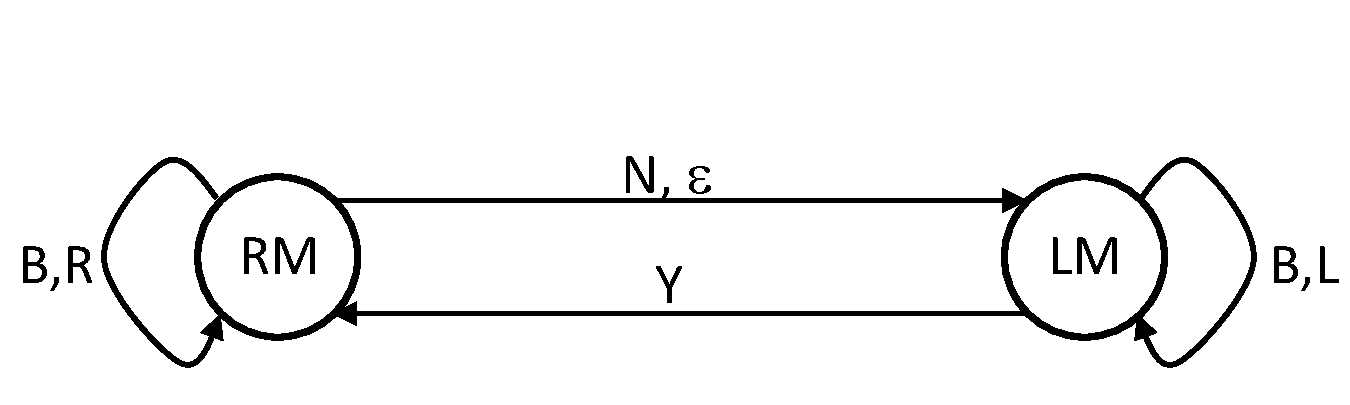
\includegraphics[scale=0.35]{YieldTypeCheckingAutomaton.pdf}
\caption{Specification for yield sufficiency}
\label{fig:YieldTypeCheckingAutomaton}
\end{figure}

\begin{figure*}
\scriptsize{
\medskip
%%%%%%%%%%%%%%%%%%%%
$
\inferrule
{
}
{\Refines;\actions \jy \skipstmt : (x, x)}
\;(\textsc{Skip})
$
\medskip
%%%%%%%%%%%%%%%%%%%%
$
\inferrule
{
}
{\Refines;\actions \jy \assert{\locExpr} : (x, x)}
\;(\textsc{Assert})
$
\medskip
%%%%%%%%%%%%%%%%%%%%
$
\inferrule
{
}
{\Refines;\actions \jy \yield{e,\lins} : (x, \RM)}
\;(\textsc{Yield})
$
\medskip
%%%%%%%%%%%%%%%%%%%%
$
\inferrule
{
P \not \in \dom(\Refines)
}
{\Refines;\actions \jy \call{P} : (x, \RM)}
\;(\textsc{Call})
$
\medskip
%%%%%%%%%%%%%%%%%%%%
$
\inferrule
{
P \in \dom(\Refines) \\ \actions(\Refines(P)) = (\rho, \alpha, B)
}
{\Refines;\actions \jy \call{P} : (x, x)}
\;(\textsc{BothMover})
$
\medskip
%%%%%%%%%%%%%%%%%%%%
$
\inferrule
{
P \in \dom(\Refines) \\ \actions(\Refines(P)) = (\rho, \alpha, R)
}
{\Refines;\actions \jy \call{P} : (\RM, \RM)}
\;(\textsc{RightMover})
$
\medskip
%%%%%%%%%%%%%%%%%%%%
$
\inferrule
{
P \in \dom(\Refines) \\ \actions(\Refines(P)) = (\rho, \alpha, L)
}
{\Refines;\actions \jy \call{P} : (x, \LM)}
\;(\textsc{LeftMover})
$
\medskip
%%%%%%%%%%%%%%%%%%%%
$
\inferrule
{
P \in \dom(\Refines) \\ \actions(\Refines(P)) = (\rho, \alpha, N)
}
{\Refines;\actions \jy \call{P} : (\RM, \LM)}
\;(\textsc{NonMover})
$
\medskip
%%%%%%%%%%%%%%%%%%%%
$
\inferrule
{
}
{\Refines;\actions \jy \async{P} : (x, \LM)}
\;(\textsc{Async})
$
\medskip
%%%%%%%%%%%%%%%%%%%%
$
\inferrule
{
x \in \{\RM,\CM\}
}
{\Refines;\actions \jy \ablock{e,\lins}{s} : (x, \CM)}
\;(\textsc{Ablock})
$
\medskip
%%%%%%%%%%%%%%%%%%%%
$
\inferrule
{
\Refines;\actions \jy \StmtStack : (x, y) \\ \Refines;\actions \jy s : (y, z)
}
{\Refines;\actions \jy \StmtStack;s : (x, z)}
\;(\textsc{Seq})
$
\medskip
%%%%%%%%%%%%%%%%%%%%
$
\inferrule
{
\Refines;\actions \jy s_1 : (x, y) \\ \Refines;\actions \jy s_2 : (x, y)
}
{\Refines;\actions \jy \ite{\locExpr}{s_1}{s_2} : (x, y)}
\;(\textsc{Ite})
$
\medskip
%%%%%%%%%%%%%%%%%%%%
$
\inferrule
{
\Refines;\actions \jy s : (x, x)
}
{\Refines;\actions \jy \while{e,\alpha}{\locExpr}{s} : (x, x)}
\;(\textsc{While})
$
\medskip
%%%%%%%%%%%%%%%%%%%%
$
\inferrule
{
\procs(P) = (\phi, \mods, \psi, \stmt) \\
\Refines;\actions \jy \stmt : (x, y)
}
{
\Refines;\actions \jy P
}
\;(\textsc{Procedure})
$
\medskip
%%%%%%%%%%%%%%%%%%%%
$
\inferrule
{
\Refines;\actions \jy \StmtStack : (x,y)
}
{
\Refines;\actions \jy (\varsL,\StmtStack) : (x,y)
}
\;(\textsc{Stack})
$
\medskip
%%%%%%%%%%%%%%%%%%%%
$
\inferrule
{
T = (\varsTL, (\varsL, \StmtStack)) \\
\Refines;\actions \jy (\varsL, \StmtStack) : (x, y)
}
{
\Refines;\actions \jy T
}
\;(\textsc{Thread})
$
\medskip
%%%%%%%%%%%%%%%%%%%%
$
\inferrule
{
\forall P \in \ProcName \setminus \dom(\Refines).\ \Refines;\actions \jy P \\\\
\forall 1 \le i \le n.\ \Refines;\actions \jy T_i
}
{
\Refines \jy (\procs, \actions, \ProcLins, \varsG, T_1 \ldots T_n)
}
\;(\textsc{Program})
$
\medskip
%%%%%%%%%%%%%%%%%%%%
}
\caption{Yield sufficiency rules}
\label{fig:yield-sufficiency}
\end{figure*}

\subsection{Program refinement}

\begin{figure*}
\scriptsize{
\medskip
%%%%%%%%%%%%%%%%%%%%
$
\inferrule
{
}
{\Refines;\RemovedActions \vdash \skipstmt \leadsto \skipstmt}
\;(\textsc{Skip})
$
\medskip
%%%%%%%%%%%%%%%%%%%%
$
\inferrule
{
}
{\Refines;\RemovedActions \vdash \assert{\locExpr} \leadsto \assert{\locExpr}}
\;(\textsc{Assert})
$
\medskip
%%%%%%%%%%%%%%%%%%%%
$
\inferrule
{
}
{\Refines;\RemovedActions \vdash \yield{e,\lins} \leadsto \yield{e,\lins}}
\;(\textsc{Yield})
$
\medskip
%%%%%%%%%%%%%%%%%%%%
$
\inferrule
{
A \not \in \RemovedActions
}
{\Refines;\RemovedActions \vdash \call{A} \leadsto \call{A}}
\;(\textsc{Atomic})
$
\medskip
%%%%%%%%%%%%%%%%%%%%
$
\inferrule
{
\Refines;\RemovedActions \vdash s \leadsto s'
}
{
\Refines;\RemovedActions \vdash \ablock{e,\lins}{s} \leadsto s'
}
\;(\textsc{Ablock-Elim})
$
\medskip
%%%%%%%%%%%%%%%%%%%%
$
\inferrule
{
\Refines;\RemovedActions \vdash s \leadsto s'
}
{
\Refines;\RemovedActions \vdash s \leadsto \ablock{e,\lins}{s'}
}
\;(\textsc{Ablock-Intro})
$
\medskip
%%%%%%%%%%%%%%%%%%%%
$
\inferrule
{
P \in \dom(\Refines)
}
{
\Refines;\RemovedActions \vdash \call{P} \leadsto \call{\Refines(P)}
}
\;(\textsc{Proc1})
$
\medskip
%%%%%%%%%%%%%%%%%%%%
$
\inferrule
{
P \not\in \dom(\Refines)
}
{
\Refines;\RemovedActions \vdash \call{P} \leadsto \call{P}
}
\;(\textsc{Proc2})
$
\medskip
%%%%%%%%%%%%%%%%%%%%
$
\inferrule
{
}
{
\Refines;\RemovedActions \vdash \async{P} \leadsto \async{P}
}
\;(\textsc{Async})
$
\medskip
%%%%%%%%%%%%%%%%%%%%
$
\inferrule
{
\Refines;\RemovedActions \vdash \StmtStack \leadsto \StmtStack'
}
{
\Refines;\RemovedActions \vdash (\varsL,\StmtStack) \leadsto (\varsL,\StmtStack')
}
\;(\textsc{Stack})
$
\medskip
%%%%%%%%%%%%%%%%%%%%
$
\inferrule
{
\Refines;\RemovedActions \vdash \StmtStack \leadsto \StmtStack' \\
\Refines;\RemovedActions \vdash \stmt \leadsto \stmt'
}
{
\Refines;\RemovedActions \vdash \StmtStack;\stmt \leadsto \StmtStack';\stmt'
}
\;(\textsc{Seq})
$
\medskip
%%%%%%%%%%%%%%%%%%%%
$
\inferrule
{
\Refines;\RemovedActions \vdash s_1 \leadsto s_1' \\
\Refines;\RemovedActions \vdash s_2 \leadsto s_2'
}
{
\Refines;\RemovedActions \vdash \ite{\locExpr}{s_1}{s_2} \leadsto \ite{\locExpr}{s_1'}{s_2'}
}
\;(\textsc{Ite})
$
\medskip
%%%%%%%%%%%%%%%%%%%%
$
\inferrule
{
\Refines;\RemovedActions \vdash s \leadsto s'
}
{
\Refines;\RemovedActions \vdash \while{e,\alpha}{\locExpr}{s} \leadsto \while{e,\alpha}{\locExpr}{s'}
}
\;(\textsc{While})
$
\medskip
%%%%%%%%%%%%%%%%%%%%
$
\inferrule
{
\Refines;\RemovedActions \vdash \stmt \leadsto \stmt'
}
{
\Refines;\RemovedActions \vdash (\phi,\mods,\psi,\stmt) \leadsto (\phi',\mods',\psi',\stmt')
}
\;(\textsc{Procedure})
$
\medskip
%%%%%%%%%%%%%%%%%%%%
$
\inferrule
{
\accessVars(\rho) \cap \Local = \emptyset \\
\alpha = ((\exists \mathit{old}(\Local), \Local.\ \alpha) \wedge \Same(\Local)) \\
}
{
\Refines;\RemovedActions \vdash (\rho,\alpha,m) \leadsto (\rho,\alpha,m)
}
\;(\textsc{Action})
$
\medskip
%%%%%%%%%%%%%%%%%%%%
$
\inferrule
{
\Refines;\RemovedActions \vdash \StmtStack \leadsto \StmtStack' \\
}
{
\Refines;\RemovedActions \vdash (\varsTL, (\varsL, \StmtStack)) \leadsto (\varsTL, (\varsL, \StmtStack')) \\
}
\;(\textsc{Thread})
$
\medskip
%%%%%%%%%%%%%%%%%%%%
$
\inferrule
{
\Prog = (\procs, \actions, \ProcLins, \varsG, T_1 \ldots T_n) \\
\Prog' = (\procs', \actions', \ProcLins', \varsG, T_1' \ldots T_n') \\
\forall 1 \le i \le n.\ \Refines;\RemovedActions \vdash T_i \leadsto T_i' \\
\forall A \not\in \RemovedActions.\ \actions(A) = \actions'(A) \\
\forall A \in \range(\Refines).\ \Refines;\RemovedActions \vdash \actions(A) \leadsto \actions(A) \\
\forall P \not\in \dom(\Refines).\ \Refines;\RemovedActions \vdash \procs(P) \leadsto \procs'(P) \\
\forall P \in \dom(\Refines).\ \ProcLins(P) = \ProcLins(\Refines(P)) \\
}
{
\Refines;\RemovedActions \vdash \Prog \leadsto \Prog'
}
\;(\textsc{Program})
$
\medskip
%%%%%%%%%%%%%%%%%%%%
}
\caption{Program refinement}
\label{fig:program-refinement}
\end{figure*}

\subsection{Soundness}

\begin{theorem}
Let $\Prog$ and $\Prog'$ be two programs.
Let $\Refines \in \ProcName \pf \ActionName$ be a partial function from procedure names to action names.
Let $\RemovedActions \in 2^{\ActionName}$ be a set of action names.
Suppose the following conditions are satisfied:
\begin{enumerate}
\item
$\vdash \Prog$ and $\vdash \Prog'$ and $\Refines;\RemovedActions \vdash \Prog \leadsto \Prog'$.
\item 
All finite executions of $\Prog'$ are safe.
\item
All infinite executions of $\Prog'$ are responsive.
\item
$\CommutativitySafe(\Prog)$.
\item
$\InterferenceFree(\Prog,\Refines)$.
\item
$\Refines \jp Prog$ and $\Refines \jr Prog$ and $\Refines \jy Prog$.
\end{enumerate}
Then all finite executions of $\Prog$ are safe.
\end{theorem}

\subsection{Responsiveness}

\[
\inferrule
{
\procs;\actions;\RefinementAny;\mods \jp \FH{e \wedge \locExpr}{s}{e} \\ e \wedge \locExpr \Rightarrow f \geq 0 \\ s \preceq (old(e \wedge \locExpr) \Rightarrow \mathit{old}(f) > f)
}
{\procs;\actions;\RefinementAny;\mods \jp \FH{e}{\while{e,\alpha,f}{\locExpr}{s}}{e \wedge \neg \locExpr}}
\;(\textsc{While})
\]


\section{Modules}
\label{sec:modules}

The technical report\cite{gc-techreport} describes a simple module system built on \civl that allows separate verification of modules,
allowing programmers to check a large program by breaking it into smaller pieces and checking the pieces independently.
A key challenge for modular verification in \civl is the checking of non-interference and commutativity.
Naively, these are whole-program judgments,
quadratically checking all pairs of actions or all pairs of yields and atomic blocks from an entire program.
To check these judgments on a per-module basis rather for a whole program,
we observe that commutativity and non-interference are trivially satisfied for operations that act on disjoint sets of global variables.
If an atomic block modifies only variables $g_1$ and $g_2$, it will not interfere with a location invariant that refers only to variables $g_3$ and $g_4$.
More generally, let each module $M$ own a set of global variables, such that each global variable is owned by exactly one module,
and decree that only $M$'s procedures and actions can access $M$'s global variables.
Statements in $M$'s procedures can only read and write $M$'s own global variables,
and $M$'s actions and location invariants can only refer to $M$'s own global variables.
(On the other hand, procedure assertions that are not checked for non-interference,
such as the $e$ in $\ablock{e}{\stmt}$,
may mention global variables from other modules,
since these assertions can neither interfere with other modules' location invariants nor be interfered with by other modules' statements.)

Note that ownership can change across refinement layers.
For example, a library module implementing locks may define a variable to represent the abstract state of a lock;
after the lock module is verified at a low layer,
another module can take ownership of the lock variable in a higher layer
(see \cite{gc-techreport} for a detailed example of ownership transfer across three layers, from a lock module to a datatype module to a client module).

\section{Experience}
\label{sec:experience}

The \civl verifier has been under development for around two years.  
Over that period, we have developed a collection of 32 benchmarks, 
ranging in size from 17 to 539 LOC, to illustrate various features of
\civl and for regression testing as we evolved the verifier.
In addition to microbenchmarks, this collection also includes
standard benchmarks from the literature such as a multiset implementation~\cite{ElmasTQ05}, 
the ticket algorithm~\cite{FarzanKP14}, 
Treiber stack~\cite{Herlihy2008}, work-stealing queue~\cite{Blumofe1999},
device cache~\cite{ElmasQT09}, and lock-protected increment~\cite{FlanaganQ03}. 
The \civl verifier is fast; the entire benchmark set verifies in 20 seconds on a standard 4-core Windows PC 
with no benchmark requiring more than a few seconds.

\subsection{Garbage collector}
We have used \civl to design and verify a realistic concurrent mark-sweep garbage collection (GC) algorithm.  
In particular, although our algorithm is based on an earlier algorithm by Dijkstra et al~\cite{dijk78}, 
it extends the earlier algorithm with various modern optimizations and embellishments to improve generality and performance.  
These extensions include lower write barrier overhead, phase-based synchronization and handshaking, 
and coordination between the GC and mutator threads during root scanning; our use of linearity aids the proof of root scanning, 
while our rely-guarantee encoding aids management of colors inside the write barrier
(which is similar to the barrier in Section~\ref{sec:overview}).
Furthermore, our encoding of the algorithm in \civl spans a wide range of abstraction, 
from low-level memory operations all the way up to high-level specifications; 
we used six levels of refinement to help hide low-level details from the high-level portions of the verification.
We believe that \civl's combination of features makes practical, for the first time, verification across such a wide range of abstraction.

\civl's support for refinement allows us to write concise specifications of the garbage collector's correctness:
to be correct, the GC must implement Allocate, ReadField, and WriteField actions that appear to act atomically,
even though in the underlying implementation,
these operations execute concurrently with the garbage collector thread and with other program threads.
The specification states that Allocate atomically adds new objects to the heap,
while ReadField and WriteField read and write fields from heap objects.
Although the garbage collector's Mark and Sweep code constitutes the bulk of the GC code,
they are hidden in the high-level specification;
they have detailed correctness specifications in the middle levels of the proof,
but the most important point at the high level is that their work not interfere with Allocate, ReadField, and WriteField.
In particular, Mark must coordinate with WriteField's write barrier,
and Sweep must not remove any objects that are still reachable by ReadField and WriteField.

The GC verification takes 60 seconds on the same 4-core Windows PC, generating and verifying 667 proof obligations. 
The bulk of this time, 54 seconds, is taken by the verification of the refinement checks from Section~\ref{sec:refinement}.
The linear type checking, the yield safety checks, and the commutativity checks take the rest of the time and are insignificant in comparison.

\subsection{Discussion of the proof}
We now put atomicity refinement techniques from the literature and
\civl in context by presenting an overview of our design
driver, the stepwise refinement of a garbage collector~\cite{gc-techreport}.
The refinement proof spans six levels of abstraction. 
Each of refinement proof relating two consecutive levels is made feasible by a different
blend of the techniques in \civl. 
% While other refinement techniques have also used garbage collectors as
% case studies, the refinement tasks tackled there bridge only one or two of the levels in 
% our refinement proof\footnote{A more specific discussion of this point
%   can be found in the technical report on the verification of the
%   garbage collector\cite{gc-techreport}.} and only target the refinement verification
% challenges apparent at those levels of the proof. 

The topmost-level description of the garbage collector provides an
idealized, abstract view of memory. 
At this level, none of the lowest-level implementation variables are
visible -- variable hiding has been used to project them away. 
In the top few levels of the garbage collector proof, invariant-based
non-interference reasoning was our primary tool, while reduction
simplified verification by enabling us to use coarser atomic actions and fewer
location invariants.  
Linear variables were used throughout the proof to model the distinct
thread identifiers for the garbage collector thread and mutator
threads, but were most instrumental in encoding single-threaded
execution in the initialization phase of the program. 
For these top few levels of our proof, rely-guarantee and separation-logic-based
approaches would have also performed well, as demonstrated by the
garbage collector proof of Liang et al.~\cite{LiangRGSim}, where
the atomicity of actions in the lower levels our proof is {\em assumed} but not verified.
An important distinguishing capability in \civl is being able to use location invariants rather than pure rely-guarantee reasoning.
This helped interactive proof at the top levels significantly.
For the mark phase of the garbage collector, we made critical use of
different invariants at different locations in procedure bodies. 
While the same non-interference argument could have been encoded in
rely-guarantee reasoning, as we had done ourselves in an earlier
version of our proof, 
it would have required the use of several additional auxiliary shared variables. 
Invariants, rely and guarantee conditions referring to such auxiliary
variables throughout the program made interactive invariant reasoning more difficult to manage. 

In the lower levels of the garbage collector proof, where
correctness of concurrent data structures and synchronization primitives were proven, we made
relatively little use of location invariants, and made heavier use of
linear variables and reduction. 
We also used variable hiding heavily to hide low-level implementation
variables. 
For lower-level refinement tasks, for instance, when verifying the correctness of a
lock-protected concurrently-accessed stack, ownership
arguments, separation logic, or \QED-style atomicity would have been
sufficient. 
But, at the higher levels of our proof, where non-interference
reasoning via invariants and linear variables was indispensable, 
atomicity alone, or ownership or separation logic arguments alone
would have run into difficulty. 

While existing techniques in the literature have as their
``sweet spot'' a few of the refinement proofs in our garbage collector
proof, they run into difficulty in others. 
More critically, they
do not facilitate layering refinement proofs, which is required for stepwise
refinement. 
Using a realistic top-down proof as \civl's design driver led us to
combine in one tool and consistent theory, the verification techniques
of linearity, reduction and non-interference reasoning in the service
of a modular refinement proof directed by the syntactic structure of
the imperative concurrent program. 

%%% SHAZ, I REMOVED THIS SECONDARY NOVELTY POINT, SINCE IT IS MADE
%%% ELSEWHERE IN THE PAPER TOO.
% For this purpose, we also devised
% novel ways to combine automata-theoretic and assertion-based
% verification, and encode the component techniques, e.g., linearity, in
% assertion-based verification.  
% %%%%%%%%% SHAZ PLEASE REFINE OR REMOVE THIS FINAL SENTENCE %%%%%%%%%%%


\section{Related work}
\label{sec:related}

Our work is the first to provide a tool and theory to support automated,
modular whole-program refinement through multiple layers, as distinct from existing work on
single-layer atomicity refinement between procedure implementations and
specifications. 
\civl combines a number of techniques in a novel manner to 
decompose the refinement task following the syntactic structure of a
program. Below, we first contrast \civl with refinement
verification techniques, and then with tools and
techniques for reasoning about concurrent programs in general. 

\subsection{Refinement-oriented verification}
Atomic action specifications have been explored by the
\calvin~\cite{FlanaganFQS05,FreundQ04} verifier. 
\civl carries out refinement verification on a procedure body
with cooperative semantics as enabled by movers types and reduction.
\calvin attempts to verify refinement directly on the preemptive
semantics, making only limited use of movers at the lowest-level
representation. 
\calvin, unlike does not support location invariants and linear
variables but incorporates rely-guarantee reasoning. 
\civl supports both location
invariants or rely-guarantee reasoning, and either technique can be
used to prove non-interference.
However, in certain cases, rely-guarantee reasoning
requires use of auxiliary (shared) variables and makes interactive
proofs difficult as was the case in our GC proof. 

\QED~\cite{ElmasQT09} is a simplifier for concurrent programs and is close in spirit to the 
refinement-oriented approach of \civl.
A key distinction between \civl and \QED is the fact that a proof step in \QED is a small rewrite in the concurrent program
that must be justified by potentially expensive reduction and invariant reasoning.
In \QED, procedures can be proven atomic only one procedure at a time, and only by
transforming their bodies by reduction to be yield free. 
The number of small proof steps directly affect both programmer
and computer effort. 
By contrast, \civl supports large proof steps, in each of which the bodies of several procedures
are automatically replaced by atomic actions, thereby lowering the cost of both interaction and automation.
The non-interference reasoning in \QED is even more limited than \calvin.
\QED supports only global invariants and does not support rely-guarantee reasoning or linear variables.

Liang et al.~\cite{LiangRGSim} present a method for verifying that procedure
bodies refine atomic specifications
The key verification approach is
rely-guarantee reasoning and the refinement (simulation) relation between
a procedure and its specification is constrained so it is preserved under
parallel composition. 
No tool support is provided. 
Authors present a (paper) GC proof, which is limited in scope compared
to ours, as their proof corresponds to a few layers of our proof. In particular,
the GC is not refined down to individual atomic memory accesses. 
Since this work uses different languages to describe the high-level
and low-level programs, it is not immediately possible to carry out a
multi-level stepwise refinement proof. 

Turon and Wand~\cite{TuronM11} use ownership disciplines and
separation logic to verify refinement of atomic specifications by 
concurrent data structure implementations. 
Rely-guarantee reasoning is
supported to provide compositionality and non-interference
arguments. 
This work targets a single refinement step between atomic
specifications for methods and their implementations. 
No tool support for this verification method is provided. 

Verifying linearizability of concurrent data structures (see, e.g.,
\cite{tacasLin,aliLin}) can be viewed as an instance of one-level of
refinement in our setting. 
\civl can be used for mechanical
verification of linearizability, as we did for the Treiber stack. 
Tools and techniques specific to verifying linearizability
cannot be easily generalized for stepwise refinement proofs
through multiple levels. 

Refinement proofs
between implementations and specifications of protocols have been
investigated using the TLA+~\cite{Lamport2004} specification
language. 
Compositional refinement proofs~\cite{AbadiAssumeGuarantee} have
been investigated in this context. 
Modular refinement proofs for hardware systems have been investigated extensively
(e.g.,~\cite{Henzinger1999,Eiriksson2000}) using the SMV~\cite{McMillan00} and Mocha~\cite{AlurHMQRT98} 
model checking tools.
To verify a concurrent, shared-memory program using such tools, one must encode
the program semantics as a state-transition system and express
verification goals in terms of this system. 
For concurrent, shared-memory
software, \civl enables reasoning on the structured, imperative
multithreaded program text rather than a logic description of the
program's state-transition relation. 
 

\subsection{Reasoning about concurrency}
In this section, we discuss foundational techniques
for combating the complexity of concurrent program verification. 
\civl and refinement techniques discussed in the previous
section have common ideas with tools and formalisms
discussed in this section, however, the latter primarily target verification of a {\em single} program rather than refinement. 
Refinement in \civl is orthogonal to these techniques, which can be aided by \civl's 
ability to connect a complex concurrent program to a simpler abstraction.

VCC~\cite{VCC} is a tool for verifying concurrent C programs.  
Chalice~\cite{LM09} is a language and modular verification tool for concurrent programs. 
VCC does not support refinement and Chalice does so only for sequential programs.  
VCC and Chalice base their invariant reasoning on objects, object ownership, and type invariants. 
Invariant reasoning in \civl is more primitive and based on predicates in yield statements. 
Although the approach in VCC and Chalice is more convenient when applicable, \civl's approach is more flexible. 
VCC and Chalice can reason sequentially about objects exclusively owned by a thread;
\civl accomplishes the same using linear variables.
Neither VCC nor Chalice support movers and reduction reasoning.

Concurrent separation logic~\cite{OHearn07} reasons about concurrency without 
explicitly checking for non-interference between threads. 
Recently, tools based on this logic that blend in explicit
non-interference reasoning (but without support for reduction and mover reasoning) have been developed~\cite{SAGL,RGSep}. 
\civl's combination of interference checking and linear variables is
an extreme example of this trend, is very general and technique-agnostic. 
We supply very primitive abstractions and let programmers mix and
match these abstractions freely to encode the non-interference reasoning style of their choice. 





\bibliographystyle{abbrv}
\bibliography{paper}

\end{document}

